\section{Observation and Calculations}

\subsection{GM Characteristics}
For the characteristics of GM Counter, the GM counter was kept in the detector stand. The $\gamma$-source was kept at a distance of 2 cm while the $\beta$-source was kept at a distance of 4 cm from the detector.The EHT voltage of the detector was varried and the number of counts was noted for 30s. For each voltage setting, the source was removed and background radiation counts was also taken. The results tabulated in Table \ref{t1} and \ref{t2} (All observational data is presented in the appendix) and are plotted (Figs. \ref{g1} and \ref{g2}) and discussed below.

\begin{figure}[H]
    \centering
    \includegraphics[width=1\columnwidth]{images/calib-gamma.eps}
    \caption{GM characteristics for $\gamma$-source Cs-137}
    \label{g1}
\end{figure}

From Fig. \ref{g1}, the starting voltage of plateau is $V_1=420$ V and the ending voltage for the plateau is $V_2=600$ V.
The plateau length is $(600-420)=190$ V. The operating voltage is hence $V_0=510$ V. Doing least square fitting for a straight line on the slope, the slope of the plateau is $(0.75 \pm 0.36)$ and the intercept is $(2592 \pm 172)$.

The percentage slope of the plateau is given by,
\begin{align} \label{perc-slope}
    \% \text{ slope } &= \frac{N_2-N_1}{N_1}\times \frac{100}{V_2-V_1}\times 100\\
    &= 2.92 \% \nonumber
\end{align}

\begin{figure}[H]
    \centering
    \includegraphics[width=1\columnwidth]{images/calib-beta.eps}
    \caption{GM characteristics for $\beta$-source Tl-204}
    \label{g2}
\end{figure}

From Fig. \ref{g2}, the starting voltage of plateau is 390 V and the ending voltage for the plateau is 600 V.
The plateau length is $(600-390)=210$ V. The operating voltage is hence 495 V. Doing least square fitting for a straight line on the slope, the slope of the plateau is $(0.11 \pm 0.06)$ and the intercept is $(286 \pm 31)$.

The percentage slope is given by Eq. \ref{perc-slope} as was found to be $3.66$\%.

\subsection{Inverse Square Law Relation}
EHT voltage is now fixed at 510V and the counting time is 60s.
By using the $\gamma$-source, obtained counts (for 60s) for the source placed at different distances $d$ from the detector (Table \ref{t3}). The corrected counts have be calculated using Table \ref{t4}.

Fitting the $R$ vs. $d$ plot (Fig \ref{g3}) using a function of the form $R=A+B/d^2$, the values of $A$ and $B$ obtained are shown in the figure.

\begin{figure}
    \centering
    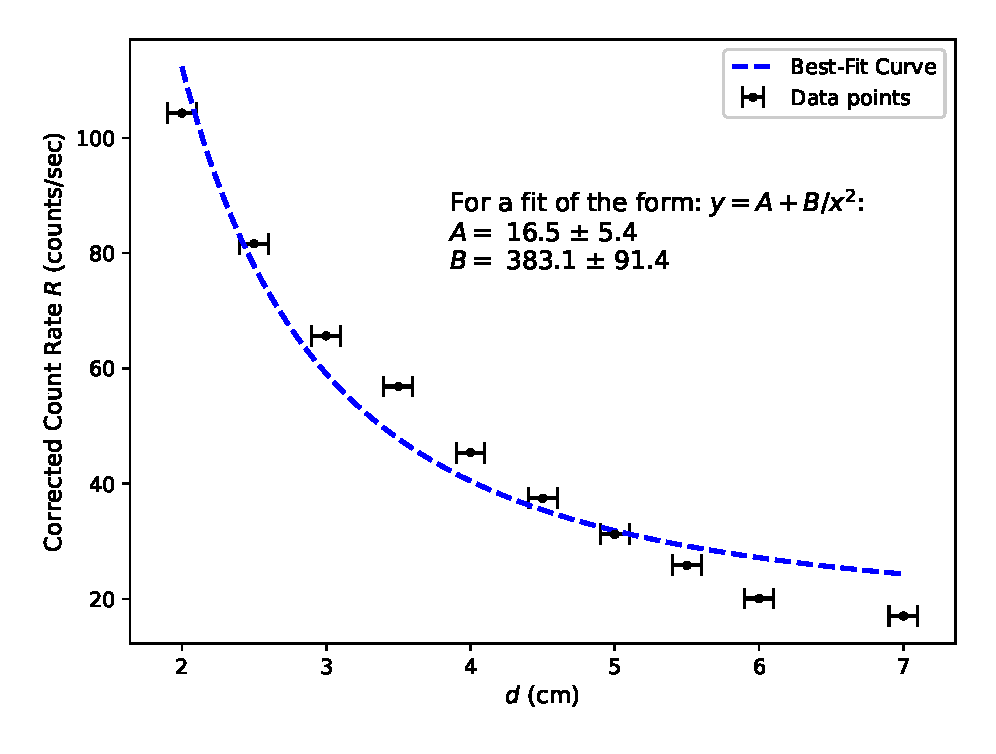
\includegraphics[width=1\columnwidth]{images/inv1.eps}
    \caption{Variation of Count Rate $R$ with distance $d$ for $\gamma$-source Cs-137}
    \label{g3}
\end{figure}

When the corrected count rate $R$ is plotted vs. $d$ by taking the log in both axes, we get Fig. \ref{g4}.
In Fig. \ref{g4}, the slope of the line indicates the exponent of $d$ w.r.t. $R$, which should ideally be equal to $-2$ (Eq. \ref{inv-eq}). Here, have obtained a slope of $-(1.60 \pm 0.05)$.
\begin{figure}
    \centering
    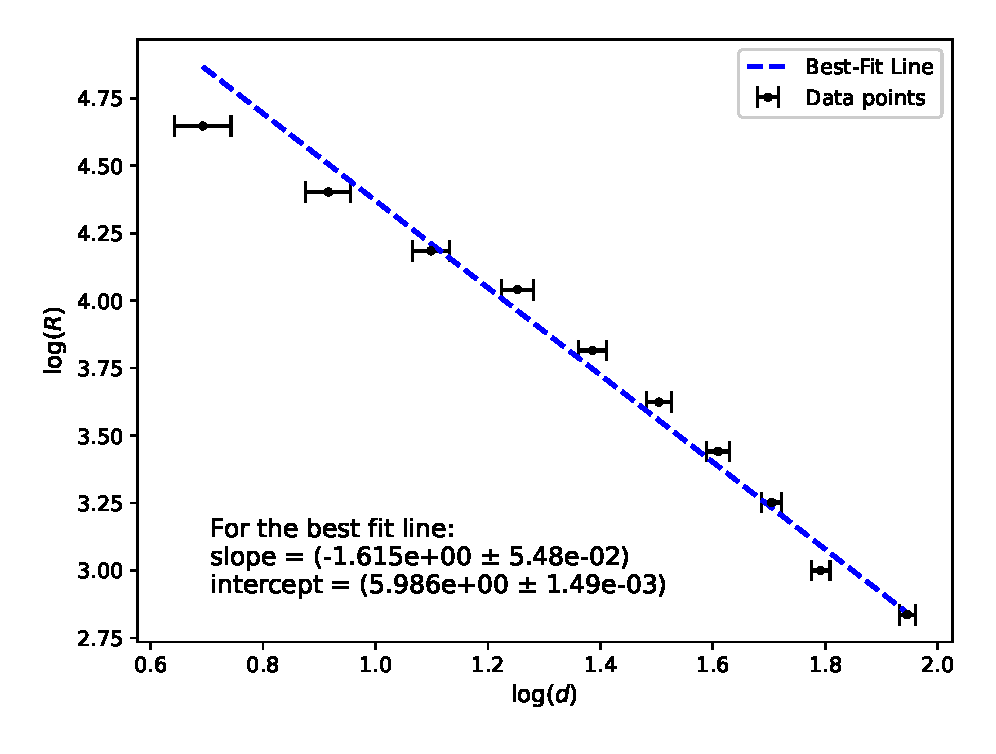
\includegraphics[width=1\columnwidth]{images/inv2.eps}
    \caption{Variation of Count Rate $R$ with distance $d$ for $\gamma$-source Cs-137 in the log scale}
    \label{g4}
\end{figure}

This means there is a significant source of error in our observations, leading to a small deviation in the inverse-square relation between count rates and distance.

We can also plot $R$ vs. $1/d^2$ to observe how closely it follows a straight line. The resultant plot and the parameters are shown in Fig. \ref{g5}. 
\begin{figure}
    \centering
    \includegraphics[width=1\columnwidth]{images/inv3.eps}
    \caption{Variation of Count Rate $R$ with $1/d^2$ for $\gamma$-source Cs-137}
    \label{g5}
\end{figure}

\subsection{Efficiency of Detection}
For a Cesium-137 source, where the initial activity in May 2016 was $A_0 = 86$ kBq, the decay constant is determined using Eq. \ref{half}.
Given that the half-life of Cesium-137 is $T_\text{half} = 30.17$ years, we can compute $\lambda$ as,

\begin{align*}
    \lambda = \frac{\ln(2)}{30.17} \approx 0.02297 \text{ year}^{-1}
\end{align*}

and the elapsed time from May 2016 to March 2025 is:

\begin{align*}
    t = 2025 - 2016 + \frac{9 \text{ months}}{12 \text{ months/yr}} = 8.75 \text{ years}
\end{align*}

\noindent Substituting these values into the decay equation, we get the activity of the Cesium-137 source at the
given time to be,
\begin{align*}
    A &= 86 \times e^{-0.02297 \times 8.75}\\
    &\approx 70.47 \text{ kBq}
\end{align*}

Using this estimated activity for Cs-137 in March 2025, we can substitute this into Eq. \ref{eff} along with $D=10$ cm and $d=1.5$ cm to obtain $R = 99.098$ s$^{-1}$. This is the fractional radiation entering the detector.

Given the net count rate $N = 14.711$ s$^{-1}$ (from Table \ref{t5}), the efficiency can be calculated as:

\begin{align*}
    E &= \frac{14.711}{99.098} \times 100 = 14.84\%
\end{align*}

\subsection{Nuclear Statistics}

\subsubsection{Background Statistics}
After removing the radioactive source from the source holder we have taken two sets of 10 readings each of the background noise with the set the preset time to 10s and 100s (Table \ref{t6}) respectively (EHT = 510 V). The bar graph for number of counts registered versus the Index Number has been shown in Fig. \ref{g6}.

\begin{figure}
    \begin{subfigure}{\linewidth}
        \centering
        \includegraphics[width=1\columnwidth]{images/spread1.eps}
        \caption{10 seconds ($\sigma = 2.62$)}
    \end{subfigure}
    % \begin{subfigure}{\linewidth}
    %     \centering
    %     \includegraphics[width=1\columnwidth]{images/spread2.eps}
    %     \caption{100 seconds ($\sigma = 7.93$)}
    % \end{subfigure}
    % \caption{Measurement of the background count for different lenghts of time. The error bars show the standard deviation in the measurements. We can see that the relative spread decreases as the measurement time increases.}
    % \label{g6}
\end{figure}
\begin{figure}
    \ContinuedFloat
    % \begin{subfigure}{\linewidth}
    %     \centering
    %     \includegraphics[width=1\columnwidth]{images/spread1.eps}
    %     \caption{10 seconds ($\sigma = 2.62$)}
    % \end{subfigure}
    \begin{subfigure}{\linewidth}
        \centering
        \includegraphics[width=1\columnwidth]{images/spread2.eps}
        \caption{100 seconds ($\sigma = 7.93$)}
    \end{subfigure}
    \caption{Measurement of the background count for different lenghts of time. The error bars show the standard deviation in the measurements. We can see that the relative spread decreases as the measurement time increases.}
    \label{g6}
\end{figure}

By comparing the two plots in Fig. \ref{g6}, we can deduce that the spread in measured values decreases as the number of pulses registered increases. Hence, the background noise reaches a stable value and shows less variation as the measurement time increases.

Now, to further demonstrate the point, we we have repeated the measurement 50 time with time of measurement 100s each. The results are tabulated in Table \ref{t7}. Fig. \ref{g7} shows the spread in the background counts. From this distribution, we can find the statistical parameters for the background counts as follows.

\begin{figure}
    \centering
    \includegraphics[width=1\columnwidth]{images/gauss-bg.eps}
    \caption{Distribution of background counts overlaid with a normal fitting function}
    \label{g7}
\end{figure}

\begin{itemize}
    \item Mean: \begin{align*}
        \bar{N} = \frac{4432}{50} \approx 89 = 0.89 \text{ counts/sec}
    \end{align*}
    \item Variance: \begin{align*}
        \sigma^2 &= \frac{1}{N}\sum^N_{i=1}(N_i-\bar{N})^2 \\ &= \frac{4467.52}{50} = 89.35
    \end{align*}
    \item Standard deviation: \begin{align*}
        \sigma &= \sqrt{89.35} = 9.45\\
        &= 0.09 \text{ counts/sec}
    \end{align*}
\end{itemize}

Here, all values have been divided by 100s to get the count rates.

\subsubsection{Distribution of Decay Counts}

For studying the number statistics, the $\beta$-source is kept at a distance of 2 cm from the detector and the counts were recorded for 25s at fixed EHT voltage of 510 V. The readings are tabulated in Table \ref{t8}.

\begin{figure}[H]
    \centering
    \includegraphics[width=1\columnwidth]{images/gauss.eps}
    \caption{Distribution of $(N_i-N)$ for $\beta$-source, where $N$ is the mean value}
    \label{g8}
\end{figure}

From Fig. \ref{g8}, we can see that the distribution tends to be Gaussian distribution as the number of measurements performed is increased. The distribution is also symmetric about the mean value. The parameters for the best-fit Gaussian distribution are shown in the figure. The mean value for $(N_i-\bar{N})$ obtained is 0 as expected. The standard deviation was obtained to be $\sigma = 24.9 \approx \sqrt{\bar{N}}$, where $\bar{N}$ is the mean value of the counts which was measured to be 632.92.

Because the mean value is large, the adjacent values of the function are not greatly different from each other. i.e., the distribution is slowly varying which is the expected behavior of a normal distribution.
